\definecolor{bg}{rgb}{0.95,0.95,0.95}
\section{Réflexion}
Fonctionnalité de base, le calcul du rayon réfléchi est relativement simple :
\begin{center}
  \inputcode[bgcolor=bg]{c++}{code/reflection.cc}
\end{center}

Le schéma de la \tsl{fig. \ref{fig:reflectionSchema}} illustre bien ce calcul. 
\begin{figure}[h]
  \begin{center}
    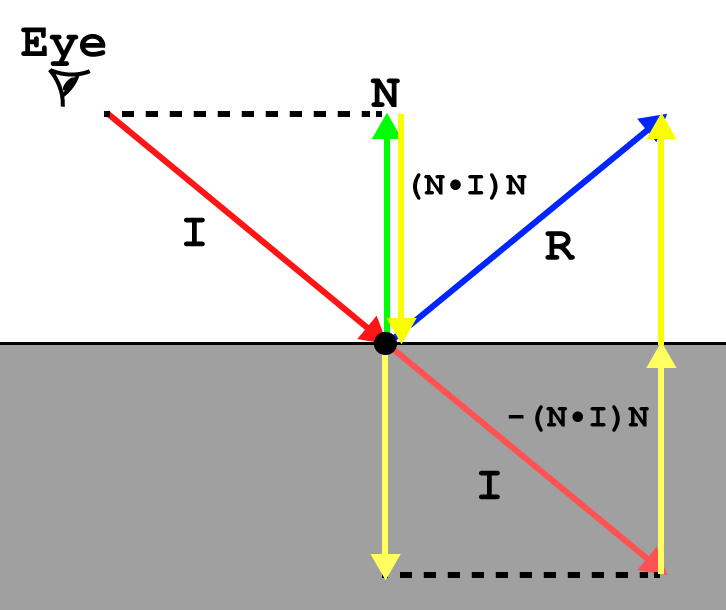
\includegraphics[width=.7\textwidth,
    keepaspectratio=true]{img/reflectionSchema}
    \label{fig:reflectionSchema}
  \end{center}
\end{figure}

\subsection{Exemple}
La \tsl{fig. \ref{fig:reflection}} présente un exemple de reflexion sur une
sphère.

\begin{figure}[h]
  \begin{center}
    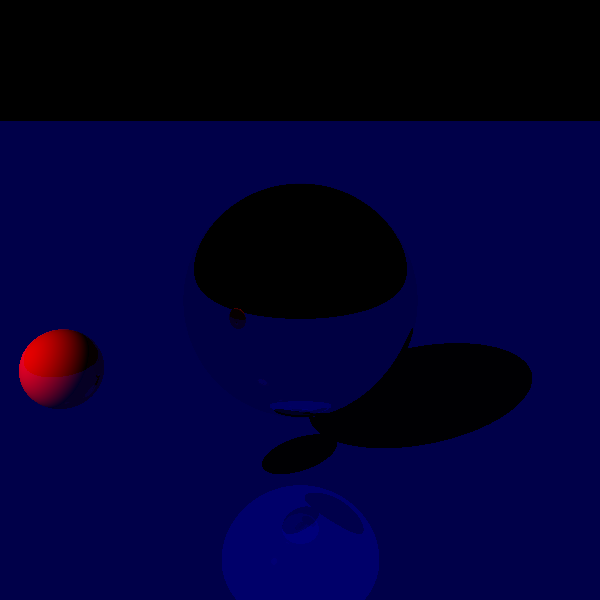
\includegraphics[width=\textwidth, keepaspectratio=true]{../../diary/10.png}
    \caption{Un exemple du rendu de la réflexion de l'environnement sur une
    sphere\label{fig:reflection}}
  \end{center}
\end{figure}

\subsection{Amélioration \& bug connu}
Aucun.
